\documentclass[11pt]{article}

% Common packages
\usepackage{amsmath}   % advanced math environments
\usepackage{amssymb}   % math symbols
\usepackage{amsthm}    % theorem/proof environments (optional, kept for later)
\usepackage{geometry}  % page margins
\usepackage{enumitem}  % better lists
\usepackage{graphicx}  % include images
\usepackage{titlesec}
\usepackage{hyperref}  % hyperlinks (keep this LAST)
\usepackage{tikz}
\usepackage{pgfplots}
\pgfplotsset{compat=1.18}

% Page setup
\geometry{margin=0.5in}
\setlist[itemize]{topsep=2pt,itemsep=2pt,parsep=0pt}

% Short labels
\newcommand{\thm}{\underline{\textbf{Thm.}} }
\newcommand{\defn}{\underline{\textbf{Def.}} }
\newcommand{\prop}{\underline{\textbf{Prop.}} }

% Title info
\title{ECON 4310 HW3}
\author{Michael Lee}

\begin{document}
\maketitle

\begin{enumerate}[label=\textbf{(\arabic*)}, leftmargin=*]
       \item \textbf{Independence Axiom.} Consider a decision maker (DM) in the expected utility framework.
       \begin{enumerate}[label=\textbf{(\alph*)}, leftmargin=*]
            \item \textit{Suppose the DM prefers lottery A to lottery B. Now take any probability p and any third lottery C. State what the Independence Axiom requires for this DM.}
            
            If the DM prefers A to B, then for some probability \(p\),
            \[
                pA + (1-p)C \succ pB + (1-p)C
            \]

            \item \textit{Find a lottery E and a probability p so that you can . . .}
            \[
                A = \{50\% \text{ of } 0, 50\% \text{ of } 100\},
                \quad
                B = \{100\% \text{ of } 40\},
                \quad 
                C = \{40\% \text{ of } 0, 50\% \text{ of } 100, 10\% \text{ of } 200\}
            \]
            \[
                D = \{80\% \text{ of } 0, 10\% \text{ of } 100, 10\% \text{ of } 200\},
                \quad
                \text{DM prefers A to B}
            \]
            \begin{enumerate}[label=\textbf{(\roman*)}, leftmargin=*]
                \item \textit{Write lottery C as a mixture of A and E, of the form C = p of lottery A, 1-p of lottery E}
                
                Define \(E = \{50\% \text{ of } 100, 50\% \text{ of } 200\}\) and \(p = 0.8\).

                \[
                    C = \{0.8 \cdot 50\% \text{ of } 0, 0.8 \cdot 50\% + 0.2 \cdot 50\% \text{ of } 100, 0.2 \cdot 50\% \text{ of } 200\}
                \]

                \item \textit{Write lottery D as a mixture of B and E of the form D = p of lottery B, 1-p of lottery E.}
                \(E\) also holds for \(D\).
                \[
                    D = \{0.8 \cdot 100\% \text{ of } 40, 0.2 \cdot 50\% \text{ of } 100, 0.2 \cdot 50\% \text{ of } 200\}
                \]
            \end{enumerate}
            \item \textit{Assuming (only) that the DM obeys EU theory (and still prefers A to B), does she prefer C to D, D to C, or can it not be determined? Provide a one sentence explanation.}
            
            C is preferred to D as C can be written as a mixture of A and E, D can be written as a mixture of B and E, and the DM prefers A to B.
        \end{enumerate}

        \item \textbf{Risk attitudes.} Consider the following two lotteries. L1 pays \$100 with probability 1. L2
        pays \$200 with probability 60\% and pays \$0 with probability 40\%.
        \begin{enumerate}[label=\textbf{(\alph*)}, leftmargin=*]
            \item \textit{What is the expected value of each lottery?}
            \[
                EV(L1) = 100 \cdot 1 = 100,
                \quad
                EV(L2) = 200 \cdot 0.6 + 0 \cdot 0.4 = 120           
            \]
            \item \textit{Which lottery would a risk-neutral DM prefer?}
            
            L2 as \(EV(L2) = 120 > EV(L1) = 100\).
            \item \textit{Which lottery would a risk-loving DM prefer?}
            
            If the risk-neutral DM prefers L2, then the risk-loving DM would prefer L2 as their utility function is convex.
            \item \textit{Which lottery would a risk-averse DM prefer?}
            
            We would need more information. Although L2 has a higher expected value, it is more risky. given the risk-averse DM's utility function is concave, they might pick L1 because it is less risky. However, we would need their utility function to determine this.
        \end{enumerate}

        \item \textbf{Risk-averse utility function.} Consider again L2 from the previous question. Draw a graph
        representing the utility function of a risk-averse decision maker (DM). Mark the points on
        the x-axis that correspond to the possible outcomes under L2. Label the utilities that the
        DM would obtain from these outcomes, u(200) and u(0), on the y-axis. Label the point on
        the graph that shows the DM’s expected utility of L2. Now find the expected value of L2 and
        label the DM’s utility of the sure amount EV(L2). Which is greater: E[u(L2)] or u(EV(L2))?
        Why?

        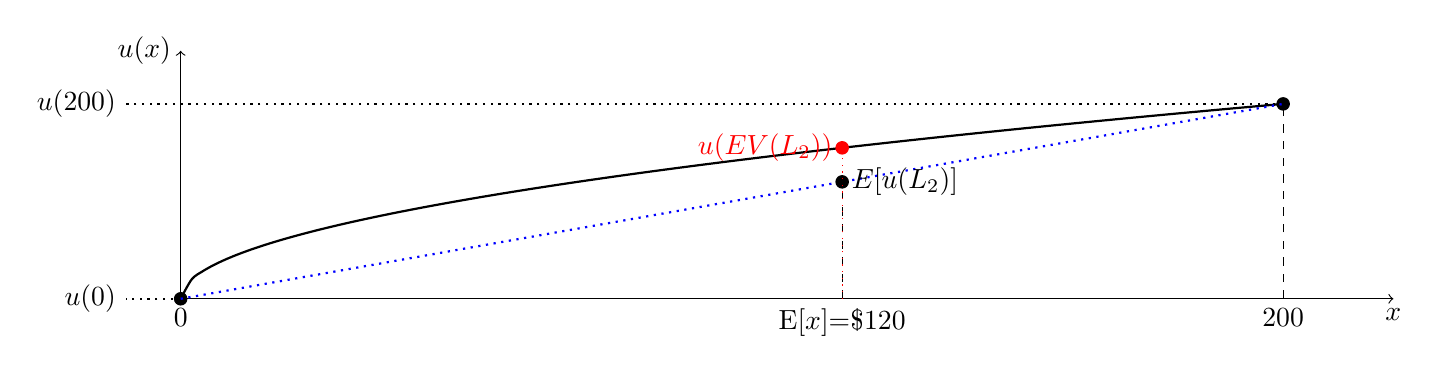
\begin{tikzpicture}[scale=0.07] % scale so 0–200 fits nicely
            % Axes
            \draw[->] (0,0) -- (220,0) node[below] {$x$};
            \draw[->] (0,0) -- (0,45) node[left] {$u(x)$};
        
            % Concave utility curve (risk-averse)
            \draw[thick,domain=0:200,smooth,samples=100] plot (\x,{2.5*sqrt(\x)});
        
            % Points for outcomes
            \pgfmathsetmacro{\uZero}{2.5*sqrt(0)}
            \pgfmathsetmacro{\uTwoHundred}{2.5*sqrt(200)}
        
            % Vertical dashed lines (from x-axis to curve)
            \draw[dashed] (0,0) node[below] {0} -- (0,\uZero);
            \draw[dashed] (200,0) node[below] {200} -- (200,\uTwoHundred);
        
            % Points on the curve
            \filldraw (0,\uZero) circle (32pt);
            \filldraw (200,\uTwoHundred) circle (32pt);
        
            % --- NEW: black dotted horizontal lines to y-axis ---
            \draw[dotted,thick] (0,\uZero) -- (-10,\uZero);
            \draw[dotted,thick] (200,\uTwoHundred) -- (-10,\uTwoHundred);
        
            % Labels on y-axis
            \node[left] at (-10,\uZero) {$u(0)$};
            \node[left] at (-10,\uTwoHundred) {$u(200)$};
        
            % Dotted blue line connecting u(0) and u(200)
            \draw[dotted,thick,blue] (0,\uZero) -- (200,\uTwoHundred);
        
            % Expected utility (E[u(L2)])
            \pgfmathsetmacro{\EUY}{0.4*\uZero + 0.6*\uTwoHundred}
            \pgfmathsetmacro{\EV}{120}
            \draw[dashed] (\EV,0) node[below] {E[$x$]=\$120} -- (\EV,\EUY);
            \filldraw (\EV,\EUY) circle (32pt) node[right] {$E[u(L_2)]$};
        
            % Utility of expected value (u(EV(L2)))
            \pgfmathsetmacro{\uEV}{2.5*sqrt(\EV)}
            \filldraw[red] (\EV,\uEV) circle (32pt) node[left,red] {$u(EV(L_2))$};
            \draw[dotted,red] (\EV,0) -- (\EV,\uEV);
        \end{tikzpicture}
        
        With loss of generality, suppose the decision maker's utlility function is \(u(x) = 2.5\sqrt{x}\).

        We know from earlier that \(EV(L2) = 120\). Thus, \(u(EV(L2)) = u(120) = 2.5\sqrt{120} \approx 27.39\).

        However, \(E[u(L2)] = 0.4 \cdot u(0) + 0.6 \cdot u(200) = 0.4 \cdot 0 + 0.6 \cdot 2.5\sqrt{200} \approx 21.21\).

        Thus, \(E[u(L2)] < u(EV(L2))\), which is evident on the graph.

        \item \textbf{Uncertainity and Risk.}
                
        This choice is not consistent with subjective EU.

        Let \(r\) be the number of red balls in Jar 2. Thus, the probability of picking a red ball in Jar 2 is \(p = \frac{r}{100}\), the number of blue balls is \(b = 100-r\), and the probability of picking a blue ball is \(1-p\).

        Suppose the DM believes \(r > 67\) and so \(p > 0.67\). Thus, the DM should prefer \(2R \succ 1R\), however, the DM prefers \(1R \succ 2R\), which is contradictory.

        If the DM believes \(r < 67\) and so \(p < 0.67\). Thus, the DM should prefer \(1R \succ 2R\), which the DM does. However, the DM also prefers \(1B \succ 2B\). The choice does not make sense as \(b > 33\), which is contradictory.

        In the case where \(r = 67\) and so \(p = 0.67\), the DM should be indifferent between \(1R\) and \(2R\) and \(1B\) and \(2B\). However, the DM strictly prefers \(1R \succ 2R\) and \(1B \succ 2B\), which is contradictory.


        Thus, these choices are not consistent with subjective EU.
        \item \textbf{Ellsburg Paradox.}
        
        \begin{enumerate}[label=\textbf{(\alph*)}, leftmargin=*]
            \item \textit{For each of the pairs of bets, determine if it can be characterized purely by objective
            risk or not.}

            Consider the first set of bets: Bet White and Bet Green.

            We know that 30 out of 90 balls are white, so \(P(\text{White}) = \frac{30}{90} = \frac{1}{3}\). We also know the number of green balls, \(g \in [0,60]\), so \(P(\text{Green}) = \frac{g}{90} \in [0, \frac{2}{3}]\). Thus, Bet White has objective risk because we know the probability of picking a white ball. However, Bet Green has subjective risk because we do not know the probability of picking a green ball. \\

            Consider the second set of bets: Bet White/Yellow and Bet Green/Yellow.

            We know that 30 out of 90 balls are white and the number of yellow balls, \(y \in [0,60]\), so \(P(\text{White}) = \frac{30 + y}{90} \in \left[\frac{1}{3}, 1\right]\). We also know that the total number of green and yellow balls, \(g + y = 60]\), so \(P(\text{Green} \cap \text{Yellow}) = \frac{g + y}{90} = \frac{60}{90} = \frac{2}{3}\). Thus, Bet Green/Yellow has objective risk because we know the probability of picking a green or yellow ball. However, Bet White/Yellow has subjective risk because we do not know the probability of picking a white or yellow ball.
        
            \item \textit{Provide an intuitive justification for the provided preferences.}
            
            In this question, the DM prefers the choices with objective risk over choices with subjective risk. Intuitively, this choice makes sense because the DM definitely knows what the probability their choice will be. However, the DM does not know the probability of their choice in the subjective risk bets.

            \item \textit{Argue that this combination of preferences is incompatible with SEU.}
            
            Let the number of green balls be \(g\) and the number of yellow balls be \(y\).
            
            Consider the case where \(g \in [31, 60]\). Thus, the DM should bet Green because \(\frac{2}{3} \geq P(\text{Green})  > P(\text{White}) = \frac{1}{3}\). Thus, they should Bet Green. However, the DM would Bet White.

            Now, consider the case where \(g \in [0, 29]\). Thus, the DM should bet White/Yellow because \(1 \geq P(\text{White} \cap \text{Yellow})  > P(\text{Green} \cap \text{Yellow}) = \frac{2}{3}\). Thus, they should White/Yellow. However, the DM would Bet Green/Yellow.

            Finally, consider the case where \(g = 30\). Here, the DM should be indifferent because \(\frac{1}{3} = P(\text{White}) = P(\text{Green})\) and \(\frac{2}{3} = P(\text{Green} \cap \text{Yellow}) = P(\text{White} \cap \text{Yellow})\).
        \end{enumerate}
        \item \textbf{Dynamic Consistency.}
        \begin{enumerate}[label=\textbf{(\alph*)}, leftmargin=*]
            \item \textit{Write down an algebraic expression for total utility \(U(c_1, c_2, c_3)\) in terms of \(\delta\)}
            \[
                U(c_1, c_2, c_3)
                = u(c_1) + \delta u(c_2) + \delta^2 u(c_3)
                = c_1 + \delta c_2 + \delta^2 c_3
            \]

            \item \textit{Consider the two consumption streams \(A = (3,0,0)\) and \(B = (0,4,0)\). For which values of \(\delta\) does the DM prefer A over B?}
            \[
                U(A) = 3 + \delta (0) + \delta^2 (0) = 3
                \quad \text{and} \quad
                U(B) = 0 + \delta (4) + \delta^2 (0) = \delta 4
            \]

            For the DM to prefer A over B, \(U(A) = 3 > U(B) = \delta 4\). Thus, \(\delta < \frac{3}{4}\).

            \item \textit{Consider the two consumption streams \(C = (0, 3, 0)\) and \(D = (0, 0, 4)\). If the DM is time
            consistent and prefers A over B, what can you conclude about her preference between
            C and D?}
            If the DM prefers A over B, then \(\delta > \frac{3}{4}\).

            Looking at \(C\) and \(D\), we have:
            \[
                U(C) = 0 + \delta (3) + \delta^2 (0) = 3\delta
                \quad \text{and} \quad
                U(D) = 0 + \delta (0) + \delta^2 (4) = 4\delta^2
            \]
            For the DM to prefer C over D, \(U(C) = 3\delta > U(D) = 4\delta^2\). Thus, \(\delta < \frac{3}{4}\). Hence, if the DM prefers A over B, then they prefer C over D.

            \item \textit{For which values of \(\delta\) does the DM prefer C over D?}

            As per the previous answer, the DM prefers C over D if \(\delta < \frac{3}{4}\).

            \item \textit{Based on this example, what do you conclude about exponential time discounting and
            time consistency?}

            This example implies that if a DM is time consistent and discounts exponentially, their preferences depend on how much time has based between two periods and the benefit received during those periods.
        \end{enumerate}

        \item \textbf{Dynamic Consistency.}
        \begin{enumerate}[label=\textbf{(\alph*)}, leftmargin=*]
            \item \textit{Write down an algebraic expression for total utility \(U(c_1, c_2, c_3)\) in terms of \(u, \beta,\) and \(\delta\).}
            \[
                U(c_1, c_2, c_3)
                = u(c_1) + \beta( \delta u(c_2) + \delta^2 u(c_3))
            \]
            \item \textit{Set \(\delta = 1\) and \(u(c) = c\). What is \(U(3,0,0)\)? What is \(U(0,4,0)\)? For which values of \(\beta\) does the DM prefer \((3,0,0)\) to \((0,4,0)\)?}
            
            \[
                \delta = 1 \text{ and } u(c) = c
                \quad \Rightarrow \quad
                U(c_1, c_2, c_3)
                = c_1 + \beta( c_2 + c_3)
            \]
            \[
                U(3,0,0) = 3 + \beta( 0 + 0) = 3
                \quad \text{and} \quad
                U(0,4,0) = 0 + \beta( 4 + 0) = 4\beta
            \]
            If the DM prefers \((3,0,0)\) to \((0,4,0)\), then \(U(3,0,0) = 3 > U(0,4,0) = 4\beta\). Thus, \(\beta < \frac{3}{4}\).
            \item \textit{What is \(U(0,3,0)\)? What is \(U(0,0,4)\)? For which values of \(\beta\) does the DM prefer \((0,3,0)\) to \((0,0,4)\)?}
            
            \[
                U(0,3,0) = 0 + \beta( 3 + 0) = 3\beta
                \quad \text{and} \quad
                U(0,0,4) = 0 + \beta( 0 + 4) = 4\beta
            \]
            If the DM prefers \((0,3,0)\) to \((0,0,4)\), then \(U(0,3,0) = 3\beta > U(0,0,4) = 4\beta\). Thus, \(0 > \beta\), which is impossible. Thus, there exists no \(\beta\) that satisfies this.
           \item \textit{For which values of \(\beta\) does the DM exhibit a preference reversal?}
           
           The DM exhibits a preference reversal in part (b) if \(\beta > \frac{3}{4}\). For part (c), there exists no \(\beta\) that causes a preference reversal.

           \item \textit{Suppose \(\beta = \frac{1}{2}\)}. If the DM is naive, will she exhibit a preference for commitment?
           
           A naive DM will not exhibit a preference for commitment because they believe their preferences later are the same as their preferences now.

           \item \textit{f the DM is sophisticated, will she exhibit a preference for commitment? How much
           would she be willing to pay in order to dictate now the choice at time 2?}

           If the DM is sophisticated, they will exhibit a preference for commitment and will pay a price such that \(U(3,0,0) < U(0,4,0)\). For \(\beta = \frac{1}{2}\), \(U(3,0,0) = 3 > U(0,4,0) = 4 \cdot \frac{1}{2} = 2\). Thus, the DM will pay a price such that \(3 - p = 2\). Thus, \(p = 1\).
        \end{enumerate}
\end{enumerate}

\end{document}
